\chapter{Infrastruktur}
\label{infrastruktur}

\section{Datenbankserver}

Beim Datenbankserver handelt es sich um einen virtuellen Server, den uns die HSR Hochschule für Technik Rapperswil für die Dauer dieser Arbeit zur Verfügung gestellt hat.
Dieser Server enthält die Installation der \kort{}-Datenbank sowie das Projektmanagementtool Redmine.
Letzteres ist die einzige kritische Anwendung auf dem Server, da sich der Rest über entsprechende Installationskripts sehr einfach und schnell neu aufbauen lässt.

Die Installation der benötigten Software kann mit dem Ubuntu Standard-Mechanismus \inlinecode{apt-\\get install} durchgeführt werden.

\begin{table}[H]
\centering
\begin{tabular}{|p{0.25\twocelltabwidth}|p{0.75\twocelltabwidth}|}
\hline 
\small{\textbf{Name}} & sinv-56055.edu.hsr.ch \\
\hline
\small{\textbf{DNS CNAME}} & kort.rdmr.ch \\
\hline 
\small{\textbf{Art des Servers}} & Virtueller Server \\
\hline 
\small{\textbf{Betriebsystem}} & Ubuntu 12.04 (LTS) \\
\hline 
\small{\textbf{Zugriff}} & Root-Zugriff via SSH \\
\hline 
\small{\textbf{Installierte Software}} & PostgreSQL 9.1, PostGIS 2.0, Redmine 2.1, MySQL 5.5, Apache Websever mit PHP 5.4 \\
\hline 
\small{\textbf{Pfade}} & Repository: \inlinecode{/home/odi/kort} \newline
Redmine: \inlinecode{/home/redmine/redmine-2.1.0} \\
\hline 
\end{tabular} 
\caption{Datenbankserver}
\label{infrastruktur-datenbankserver-tabelle}
\end{table}

\subsection{Datenbank-Webservice}
Der Zugang auf die Datenbank von aussen läuft ausschliesslich über den \gls{REST}-Webservice.
Für den Betrieb dieses Dienstes ist eine Apache Webserver Installation mit PHP-Unterstützung (mindestens PHP 5.3) erforderlich.

Für den Betrieb des Webservice ist das \kort{}-Repository auf dem Server geklont.
Anschliessend muss noch ein Symlink angelegt werden, um das Skript korrekt aufrufen zu können:

\inlinecode{\$ ln -s /home/odi/kort/server/webservices /var/www/webservices}

Der Webservice wird in Abschnitt \ref{webservice-database} genauer beschrieben.

\subsection{Redmine}
Die Installation von Redmine verlangt es, einen neuen Benutzer \inlinecode{redmine} auf dem Server anzulegen.
Danach muss die Software nur noch auf den Server kopiert werden und der Installationsanleitung gefolgt werden.
Diese ist in der Datei  \inlinecode{/server/redmine/redmine\_install.md} zu finden.

\subsubsection{Backup}
Die Daten von Redmine werden über zwei Skripts täglich gesichert. 
Das Skript \inlinecode{redmine\_\\backup.sh} kümmert sich darum, alle Backup-Daten täglich auf dem virtuellen Server zu sammeln und an einem zentralen Ort zu speichern.

Mit dem zweiten Skript \inlinecode{sync\_backup.sh} kann dann das zuvor erstellte Backup auf beliebige andere Systeme verteilt werden.
In unserem Fall haben wir das Skript auf unseren Laptops eingerichtet und so täglich die aktuellen Daten gesichert.


\section{Webserver (Heroku)}

Bei \brand{Heroku}\footnote{\url{http://www.heroku.com/}} handelt es sich um einen kostenlosen Dienst, welcher eine Deploymentumgebung für verschiedenste Plattformen anbietet. 
Der Dienst hat eine Schnittstelle, über welche sich automatisiert Applikationen erstellen lassen. Die Datenübertragung läuft dann über \gls{Git}.

\begin{table}[H]
\centering
\begin{tabular}{|p{0.25\twocelltabwidth}|p{0.75\twocelltabwidth}|}
\hline 
\small{\textbf{Art des Servers}} & Server in der \gls{Cloud} \\
\hline 
\small{\textbf{Betriebsystem}} & Ubuntu \\
\hline 
\small{\textbf{Zugriff}} & Daten via \gls{Git}, Befehle via Kommandozeilen-\gls{API} (\brand{Heroku-Toolbelt}) \\
\hline 
\small{\textbf{Installierte Software}} & Apache, \kort{} \gls{WebApp} \\
\hline 
\end{tabular} 
\caption{Server bei Heroku}
\label{infrastruktur-heroku-tabelle}
\end{table}

Die Entscheidung, den Webserver von \brand{Heroku} zu wählen, ist dadurch begründet, dass uns dies die grösstmögliche Freiheit bietet. 
\brand{Heroku} bietet bereits eine hervoragende \gls{API}, welche sich über das Kommandozeilen-Toolset \brand{Heroku-Toolbelt} steuern lässt.
Dies erlaubt es, beliebig viele Applikationen automatisiert zu erstellen.
Auch für den Betrieb bietet das \gls{API} viele Möglichkeiten zur Fernwartung an (SSH-Zugang, Logs, Prozessorauslastung).

\section{Deployment}
Am Deployment der Applikation sind mehrere Systeme beteiligt. 
Alle Änderungen werden von den Entwicklern via \gls{Git} zu \brand{GitHub}\footnote{\url{http://github.com}} übertragen. 
Auf \brand{GitHub} gibt es sogenannte \emph{Hooks}, die man aktivieren kann. 
Dabei handelt es sich um weitere Aktionen, welche durch verschiedene Ereignisse ausgelöst werden können. 
In unserem Fall haben wir einen \emph{post-commit Hook} aktiviert, welcher dem \gls{ci} Dienst \brand{Travis-CI}\footnote{\url{http://travis-ci.org}} Bescheid gibt, wenn neue Änderungen auf \brand{GitHub} eingetroffen sind.

Nach einem erfolgreichen Build werden die Resultate an \brand{Heroku} gesendet.
Zusätzlich wird der Datenbankserver über die Änderungen notifiziert, worauf dieser sich selbst aktualisiert.

\begin{figure}[H]
	\centering
	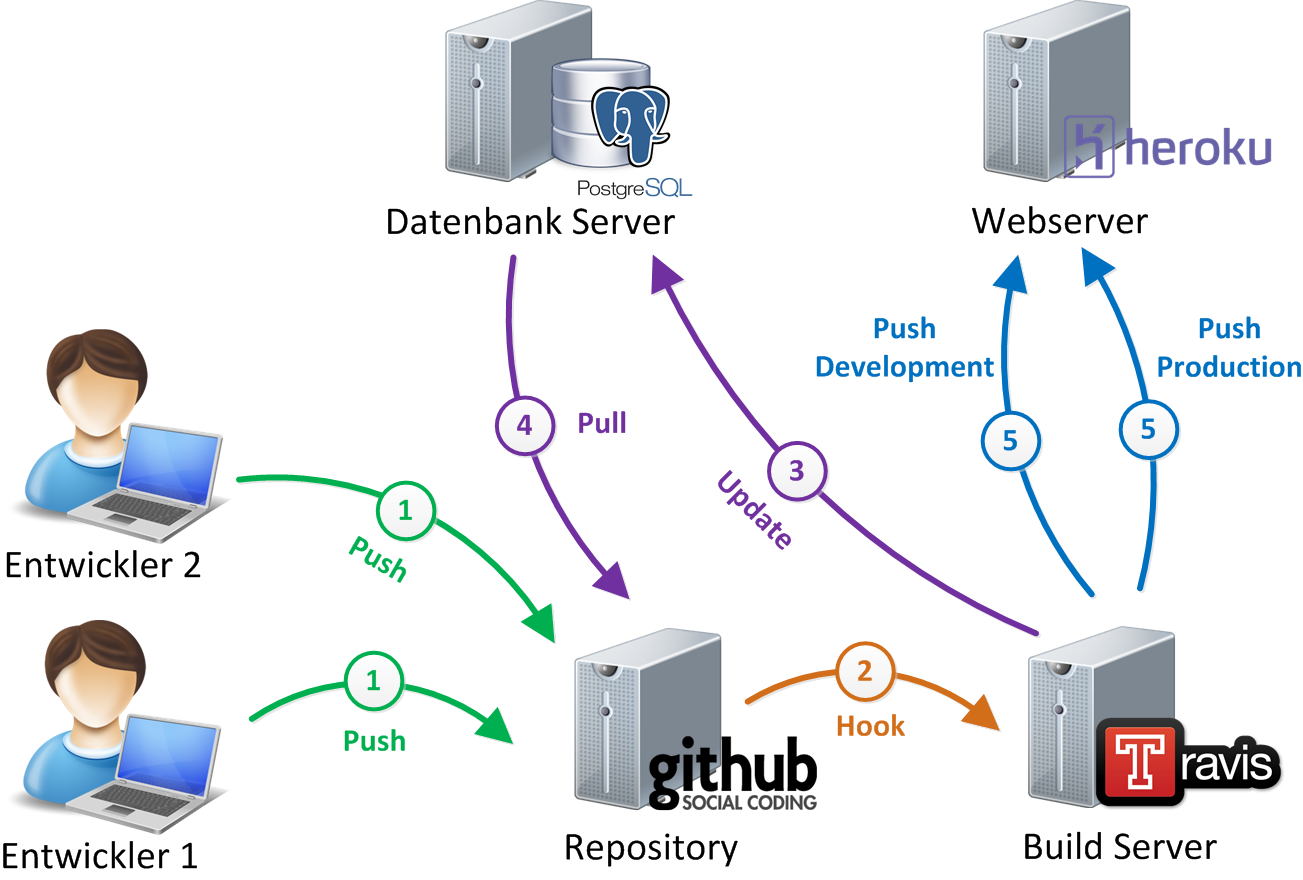
\includegraphics[scale=0.35]{images/implementation/backend/kort-development}
	\caption{Entwicklungsprozess von \kort{}}
	\label{image-kort-development}
\end{figure}

\subsection{Travis CI}
Auf \brand{Travis} läuft der Build, welcher durch die Konfigurationsdatei \inlinecode{.travis.yml} gesteuert ist. Darin lassen sich die Schritte sowie die Umgebung für Builds definieren.
Für jede Umgebung wird ein separater Build ausgelöst.
Somit lassen sich bequem verschiedene Versionen mit unterschiedlichen Umgebungen testen.
Daraus entsteht eine sogenannte Build-Matrix, welche bei jedem Build durchlaufen wird (siehe Tabelle \ref{infrastruktur-build-matrix}).

\begin{table}[H]
\centering
\begin{tabular}{|p{0.15\threecelltabwidth}|p{0.425\threecelltabwidth}|p{0.425\threecelltabwidth}|}
\hline 
 & \textbf{Test} & \textbf{Produktion} \\
\hline 
\textbf{PHP 5.3} & Build und Test & Build und Test \\
\hline 
\textbf{PHP 5.4} & Build, Test und Deployment auf \url{http://kort-dev.herokuapp.com} & Build, Test und Deployment auf \url{http://kort.herokuapp.com} \\
\hline 
\end{tabular} 
\caption{Build-Matrix von Travis CI}
\label{infrastruktur-build-matrix}
\end{table}

Ein Travis-Build läuft immer in einer neuen virtuellen Umgebung, so dass strikt nach dem Prinzip des \emph{\glslink{Bootstrapping}{Bootstrappings}} vorgegangen werden muss.
Das bedeutet, es muss möglich sein, die Applikation ohne Vorkenntnisse zu installieren.
Dies hilft, den Installationsprozess genau festzuhalten.

Am Ende des Build-Vorgangs wird die \gls{WebApp} schliesslich zu Heroku übertragen.

\subsection{Konfiguration über .travis.yml}
Die \inlinecode{.travis.yml} Datei ist die Konfigurationsdatei von \brand{Travis CI}.
Darin wird die Build-Matrix festgelegt sowie die die einzelnen Schritte des Builds definiert.

Vor dem eigentlichen Build wird die Umgebung aufgesetzt und die benötigte Software installiert (Zeilen 19-34 in Code-Ausschnitt \ref{travis-yml}).

\lstset{language=XML}
\begin{lstlisting}[float, caption=Die Travis CI Konfigurationsdatei .travis.yml, label=travis-yml]
language: php

php:
  - 5.3
  - 5.4

env:
  global:
    - CI_HOME=`pwd`/odi86/kort
    - DEPLOY="true"
    - BUILD_DIR=`pwd`/build_heroku
    - secure: "EIn+Rm7OxX8OKygBRBCaSTOqFGcBMWu5kHdKqSxOmHRJYjxuMOJpKV+rnyep\n+RsyFDx2Z9yKlqRRS4cpZh7M6wwC63EV46+7aWtzzTjnbMZfVzLQA9EmaEU4\nYMsKGtpQk2mhvaNKd3UbEpDl0Zq74NnAY0zipx0l02UymcFnZEc="
    - secure: "cOmMBP4UyklRC0nfeTZsX/NV4GhMBT+AntUmlWxXS5Rj2yrNcmNc7320gNm5\nCLSVRYyk7/8feyUEMznWrUn/62htZp0tEBAWtXg86dgIZgH4HPy9l2pKuSsH\nxZTHgjUJI7JOuyLG4ID9D5maVLE35UWag/NEtcRVy5QXLZOrs0M="
  matrix:
    - TARGET_ENV="dev"
    - TARGET_ENV="prod"

before_script:
  - gem install sass
  - gem install compass
  - gem install jsduck
  - wget -qO- https://toolbelt.heroku.com/install-ubuntu.sh | sh >/dev/null 2>&1
  - sudo npm install -g grunt >/dev/null 2>&1
  - pear install PHP_CodeSniffer && phpenv rehash
  - sudo pear channel-discover pear.survivethedeepend.com
  - sudo pear channel-discover hamcrest.googlecode.com/svn/pear
  - sudo pear channel-discover pear.phpdoc.org
  - sudo pear install --alldeps deepend/Mockery
  - sudo pear install phpdoc/phpDocumentor-alpha && phpenv rehash
  - sudo apt-get install graphviz
  - export PATH="$PATH:$CI_HOME:/usr/local/heroku/bin"
  - curl http://kort.rdmr.ch/webservices/update/git
  - mv $CI_HOME/server/php/Webservice/Database/DbConfig.example.php $CI_HOME/server/php/Webservice/Database/DbConfig.php

script: ant -f build_kort.xml build

after_script: bash $CI_HOME/server/heroku/heroku.sh
\end{lstlisting}

\subsubsection{Build-Matrix}
Die Build-Matrix bestimmt, welche Builds mit welchen Parametern ausgeführt werden.
Dabei wird gemäss definierten Sprachversionen (Zeilen 3-5 im Code-Ausschnitt \ref{travis-yml}) und Umgebungsvariablen (Zeilen 15-17) ein Build ausgeführt.
Daneben gibt es noch eine Reihe von globalen Umgebungsvariablen, welche in allen Builds verwendet werden.
In unserem Fall werden also vier Builds ausgeführt, mit jeweils PHP 5.3 und PHP 5.4 für die Test- und die Produktionsumgebung.

\subsubsection{Verschlüsselte Umgebungsvariablen}
Die Einträge mit \emph{secure} sind verschlüsselte Einträge, welche bei der Ausführung des Builds wieder entschlüsselt werden\footnote{\url{http://about.travis-ci.org/docs/user/build-configuration/\#Secure-environment-variables}}.
Auf diese Art lassen sich geheime Informationen wie \gls{API}-Schlüssel schützen.

In unserem \inlinecode{.travis.yml} kommt dies zweimal zum Einsatz:
\begin{enumerate}
\item \brand{Heroku} \gls{API}-Key, mit welchem sich beliebige Aktionen auf \brand{Heroku} durchführen lassen
\item \kort{} DB \gls{API}-Key, welcher den Datenbank-Webservice (siehe Abschnitt \ref{webservice-database}) vor fremden Zugriffen schützt
\end{enumerate}

\subsection{Apache Ant}
Das Build-Skript ist mit Apache Ant geschrieben.
Es beinhaltet alle Targets und Kombinationen davon, um einen kompletten oder teilweisen Build durchzuführen.

Derzeit werden bei einem vollständigen Build folgende Schritte durchlaufen:
\begin{enumerate}
\item Aus den SCSS-Quelldateien wird CSS generiert
\item Die JavaScript- und PHP-Dateien werden auf ihren Code Style geprüft
\item Anschliessend wird die Code-Dokumentation generiert
\item Zum Schluss werden noch die Unit Tests ausgeführt
\end{enumerate}

\subsubsection{GruntJS}
\label{gruntjs}
Die JavaScript spezifischen Build-Aufgaben werden von Ant an \brand{GruntJS}\footnote{\url{http://gruntjs.com/}} abgegeben.
Dieses Tool hat wiederum sein eigenes Konfigurationsfile \inlinecode{grunt.js}.
Darin sind Tasks beschrieben, welche auf den Code angewendet werden sollen.

In unserem Fall brauchen wir Grunt für zwei Aufgaben: JavaScript-Tests ausführen und JSHint auf sämlichen JavaScript Quellcode anwenden.

Bei \brand{JSHint}\footnote{\url{http://www.jshint.com/docs/}} handelt es sich um ein Linting-Werkzeug, welches mit diversen Optionen konfiguriert werden kann.
Das Ziel ist, dass der Code einheitlich wird und ein gewisser Code-Standard eingehalten wird.
Der Code wird dadurch besser lesbar und weniger fehleranfällig.

Die Unit Tests sind mit \brand{QUnit}\footnote{\url{http://qunitjs.com/}} erstellt und werden mit dem headless Browser \brand{PhantomJS}\footnote{\url{http://phantomjs.org/}} durchgeführt.
Dies ermöglicht es, auf einfache Art und Weise Frontend-Tests während dem Build durchzuführen.

\subsubsection{PHP\_CodeSniffer (PHPCS)}
\label{phpcs}
Der \brand{PHP\_CodeSniffer}\footnote{\url{http://pear.php.net/manual/en/package.php.php-codesniffer.php}} ist ein Linting-Tool für PHP.
Unser Code verwendet den Standard PSR-2\footnote{\url{https://github.com/php-fig/fig-standards/blob/master/accepted/PSR-2-coding-style-guide.md}}, welcher noch mit einigen Regeln zu PHPDoc-Kommentaren angereichert wurde.

Dadurch ist sichergestellt, dass der Code sauber ist und keine unerwarteten Seiteneffekte auftreten.
PHPCS lässt sich direkt in die Entwicklungsumgebung integrieren, so dass direkt beim Schreiben des Codes der Style überprüft werden kann.
